\documentclass[tikz,border=8pt]{standalone}

\usepackage{amsmath}
\usetikzlibrary{arrows.meta,positioning,calc}

\definecolor{tmfblue}{HTML}{3575A7}
\definecolor{tmfteal}{HTML}{3F9483}
\definecolor{tmforange}{HTML}{D98254}
\definecolor{tmfgray}{HTML}{65717E}

\begin{document}
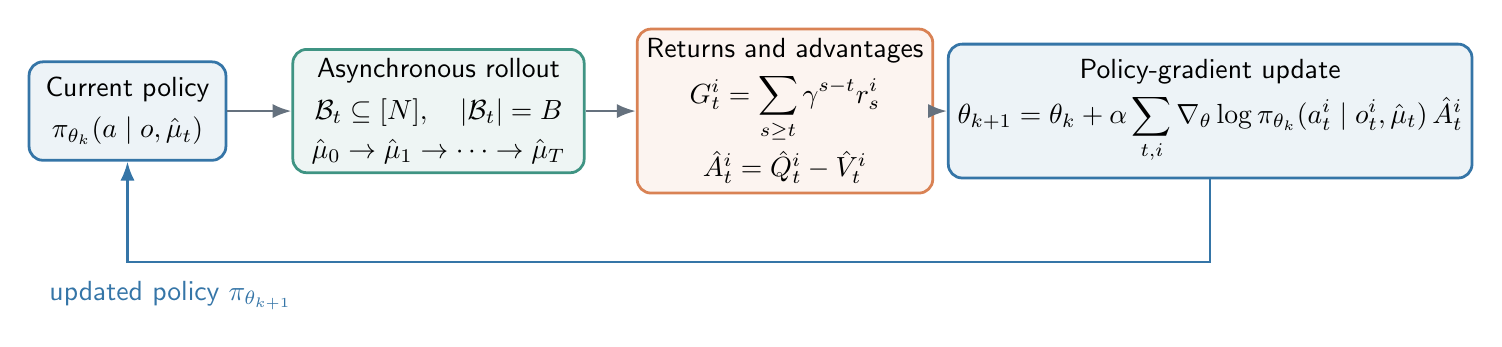
\begin{tikzpicture}[
    font=\sffamily,
    >=Latex,
    policy/.style={
        draw=tmfblue,
        fill=tmfblue!9,
        rounded corners=5pt,
        minimum width=2.5cm,
        minimum height=1.25cm,
        align=center,
        line width=1pt
    },
    rollout/.style={
        draw=tmfteal,
        fill=tmfteal!9,
        rounded corners=5pt,
        minimum width=3.7cm,
        minimum height=1.55cm,
        align=center,
        line width=1pt
    },
    data/.style={
        draw=tmforange,
        fill=tmforange!9,
        rounded corners=5pt,
        minimum width=3.65cm,
        minimum height=1.55cm,
        align=center,
        line width=1pt
    },
    update/.style={
        draw=tmfblue,
        fill=tmfblue!9,
        rounded corners=5pt,
        minimum width=5.55cm,
        minimum height=1.7cm,
        align=center,
        line width=1pt
    },
    flow/.style={-{Latex[length=2.4mm]},line width=0.9pt,tmfgray}
]

% Current policy
\node[policy] (policy) at (0,0) {
    Current policy\\[3pt]
    $\pi_{\theta_k}(a\mid o,\hat\mu_t)$
};

% Forward rollout
\node[rollout] (rollout) at (3.95,0) {
    Asynchronous rollout\\[3pt]
    $\mathcal B_t\subseteq[N],\quad |\mathcal B_t|=B$\\[2pt]
    $\hat\mu_0\rightarrow\hat\mu_1\rightarrow\cdots\rightarrow\hat\mu_T$
};

% Collected data and advantage estimates
\node[data] (data) at (8.35,0) {
    Returns and advantages\\[3pt]
    $G_t^i=\displaystyle\sum_{s\ge t}\gamma^{s-t}r_s^i$\\[2pt]
    $\hat A_t^i=\hat Q_t^i-\hat V_t^i$
};

% Policy-gradient update
\node[update] (update) at (13.75,0) {
    Policy-gradient update\\[3pt]
    $\displaystyle
    \theta_{k+1}=\theta_k+\alpha
    \sum_{t,i}
    \nabla_\theta\log\pi_{\theta_k}
    (a_t^i\mid o_t^i,\hat\mu_t)\,\hat A_t^i$
};

% Main learning flow
\draw[flow] (policy.east) -- (rollout.west);
\draw[flow] (rollout.east) -- (data.west);
\draw[flow] (data.east) -- (update.west);

% Updated policy starts the next iteration
\draw[flow,tmfblue]
    (update.south) -- ++(0,-1.05) -|
    node[pos=0.48,below=3pt,text=tmfblue] {updated policy $\pi_{\theta_{k+1}}$}
    (policy.south);

\end{tikzpicture}
\end{document}
